\documentclass{article}

\usepackage[margin=1in]{geometry}
\usepackage{fancyhdr}
\usepackage{csquotes}
\usepackage{marginnote}
\usepackage[style=apa]{biblatex}
\usepackage{xr}
\usepackage{enumitem}
\usepackage{siunitx}
\usepackage{scrextend}
\usepackage[bottom]{footmisc}
\usepackage{tikz}
\usepackage{amsmath,amssymb}
\usepackage{bm}
\usepackage{physics,mathtools}
\usepackage[hidelinks]{hyperref}

\fancypagestyle{main}{
    \fancyhf{}
    \fancyhead[L]{\leftmark}
    \fancyhead[R]{PHYS 13300}
    \fancyfoot[R]{Labalme \thepage}
}
\fancypagestyle{plain}{
    \renewcommand{\headrulewidth}{0pt}
    \fancyhead{}
}

\MakeOuterQuote{"}

\reversemarginpar

\setitemize[3]{label={\scriptsize$\blacksquare$}}

\sisetup{per-mode=symbol}

\deffootnotemark{\textsuperscript{\textup{[}\thefootnotemark\textup{]}}}
\deffootnote[2.1em]{0em}{0em}{\textsuperscript{\thefootnote}}

\colorlet{orx}{orange!70!yellow!88!black}
\colorlet{orz}{orx!25}
\colorlet{blx}{cyan}
\colorlet{pix}{magenta}
\colorlet{grx}{green!65!black}

\addbibresource{../main.bib}
\DefineBibliographyStrings{english}{bibliography={References}}

\usepackage{subfiles}

\pagestyle{main}
\renewcommand{\leftmark}{Lab Report 2 (Interference and Diffraction)}

\begin{document}




\section{Two Source Interference Questions}
\marginnote{8/21:}This investigation uses the \href{https://phet.colorado.edu/sims/html/wave-interference/latest/wave-interference_en.html}{Wave Interference PhET Simulation}.
\begin{enumerate}
    \item Choose a particular wavelength of light and a specific source separation (and record them in your report).
    \begin{itemize}
        \item Qualitatively (that is, without using numbers) where do you see maxima on the screen? Where do you see minima?
        \item Do the positions of these maxima and minima move as you change the wavelength?
        \begin{itemize}
            \item If so, how? (Be specific. As you increase wavelength, what happens? As you decrease?)
            \item Do any of the maxima or minima stay put as you change wavelength?
        \end{itemize}
        \item What happens as you increase or decrease the source separation? (Again, be specific.)        
    \end{itemize}
    \begin{proof}[Answer]
        I'm choosing green light with source separation of $\SI{1500}{\nano\meter}$.\par
        I see the maxima at the center, and then one band above and below. The minima are in between. The bands get closer together as wavelength decreases and vice versa. The central maximum stays put. As you increase the source separation, you get more bands.
    \end{proof}
    \item Now let's get quantitative. For one wavelength and separation, find a \textbf{maximum} on the screen\dots
    \begin{itemize}
        \item Measure the light's wavelength and estimate the uncertainty.
        \item Measure the distance from each light source to the maximum and estimate the uncertainty.
        \item What is the difference between the distances from each source?
        \item How does this path length difference compare to the wavelength of the light?        
    \end{itemize}
    \begin{proof}[Answer]
        Again, I'm choosing green light with source separation of $\SI{1500}{\nano\meter}$.\par
        From crest to crest, the in-simulation ruler tells us that the wavelength appears to be about $587.6\pm\SI{50}{\nano\meter}$. The distance from each light source to the central maximum appears to be about $5073.2\pm\SI{50}{\nano\meter}$. The difference between the distances from each source is zero. The path length difference is negligible compared to the wavelength of the light.
    \end{proof}
    \item Now repeat for one \textbf{minimum} on the screen\dots
    \begin{itemize}
        \item Measure the distance from each light source to the minimum and estimate the uncertainty.
        \item What is the difference between the distances from each source?
        \item How does this path length difference compare to the wavelength of the light?        
    \end{itemize}
    \begin{proof}[Answer]
        The distances from each light source to the first lateral minimum appears to be about $5000.0\pm\SI{50}{\nano\meter}$ and $5225.6\pm\SI{50}{\nano\meter}$. The difference between the distances from each source is $225.6\pm\SI{50}{\nano\meter}$. The path length difference is about one-sixth the wavelength of the light.
    \end{proof}
    \item Putting all this investigation together\dots
    \begin{itemize}
        \item What mathematical relationship between the two path lengths do we need to see constructive interference (a maximum) and what relationship do we need for destructive interference (a minimum)?
    \end{itemize}
    \begin{proof}[Answer]
        For constructive interference, we require that $\Delta r=n\lambda$ where $n\in\N$. On the other hand, for destructive interference, we require that $\Delta r=(n+\frac{1}{2})\lambda$ where $n\in\N$.
    \end{proof}
\end{enumerate}



\section{Microwave Interferometer Wavelength}
\textbf{Materials}: This investigation uses \href{https://youtu.be/OxkM7_dpSpk}{this YouTube Video}.\par
\textbf{Constants}: The wave frequency and speed of light are held constant. Thus, the wavelength (which we want to measure) is also technically constant.\par
\textbf{Experiment}: To determine the wave length, a microwave interferometer was set to varying distances and points of constructive interference were observed. The distance the microwave interferometer had to be adjusted to reach adjacent points of constructive interference is directly proportional to the wavelength. Indeed, the distance the ruler moves between peaks shifts the outgoing and incoming wave by one wavelength. However because both the reflected wave is getting longer and the incoming wave is getting shorter, the compound effect is that the distance between any two adjacent peaks is equal to half a wavelength. Thus, we will average the distances between every pair of adjacent peaks, find the standard deviation, and multiply by 2 to yield the wavelength.\par
\textbf{Data}:
\begin{table}[h!]
    \centering
    \renewcommand{\arraystretch}{1.4}
    \begin{tabular}{c|c}
                & Ruler Position ($\si{\centi\meter}$)\\
        \hline
        Peak 1 & 94.5\\
        Peak 2 & 93.2\\
        Peak 3 & 91.7\\
        Peak 4 & 90.3\\
        Peak 5 & 88.8\\
        Peak 6 & 87.3\\
        Peak 7 & 85.9\\
        Peak 8 & 84.5\\
        Peak 9 & 83.1\\
        Peak 10 & 81.6\\
        Peak 11 & 80.2\\
        Peak 12 & 78.7\\
    \end{tabular}
    \caption{Ruler position at points of constructive interference.}
    \label{fig:exp1data}
\end{table}\par
\textbf{Analysis}:\\
\begin{align*}
    \frac{\lambda}{2} &= \frac{(94.5-93.2)+(93.2-91.7)+\cdots+(80.2-78.7)}{11}\\
    &= \frac{94.5-78.7}{11}\\
    &= \SI{1.44}{\centi\meter}
\end{align*}
\begin{align*}
    \frac{\delta\lambda}{2} &= \sqrt{\frac{((94.5-93.2)-1.44)^2+((93.2-91.7)-1.44)^2+\cdots+((80.2-78.7)-1.44)^2}{11}}\\
    &= 0.064
\end{align*}
Therefore,
\begin{equation*}
    \lambda = 2.88\pm\SI{0.128}{\centi\meter}
\end{equation*}\par
\textbf{Reflection}: This value for the wavelength is not statistically significantly different from the predicted value of $\lambda=\frac{\SI{3e10}{\centi\meter\per\second}}{\SI{10.5e9}{\per\second}}=\SI{2.86}{\centi\meter}$.



\section{Single Slit Diffraction Analysis}
\textbf{Materials}: I analyzed the following image.
\begin{figure}[h!]
    \centering
    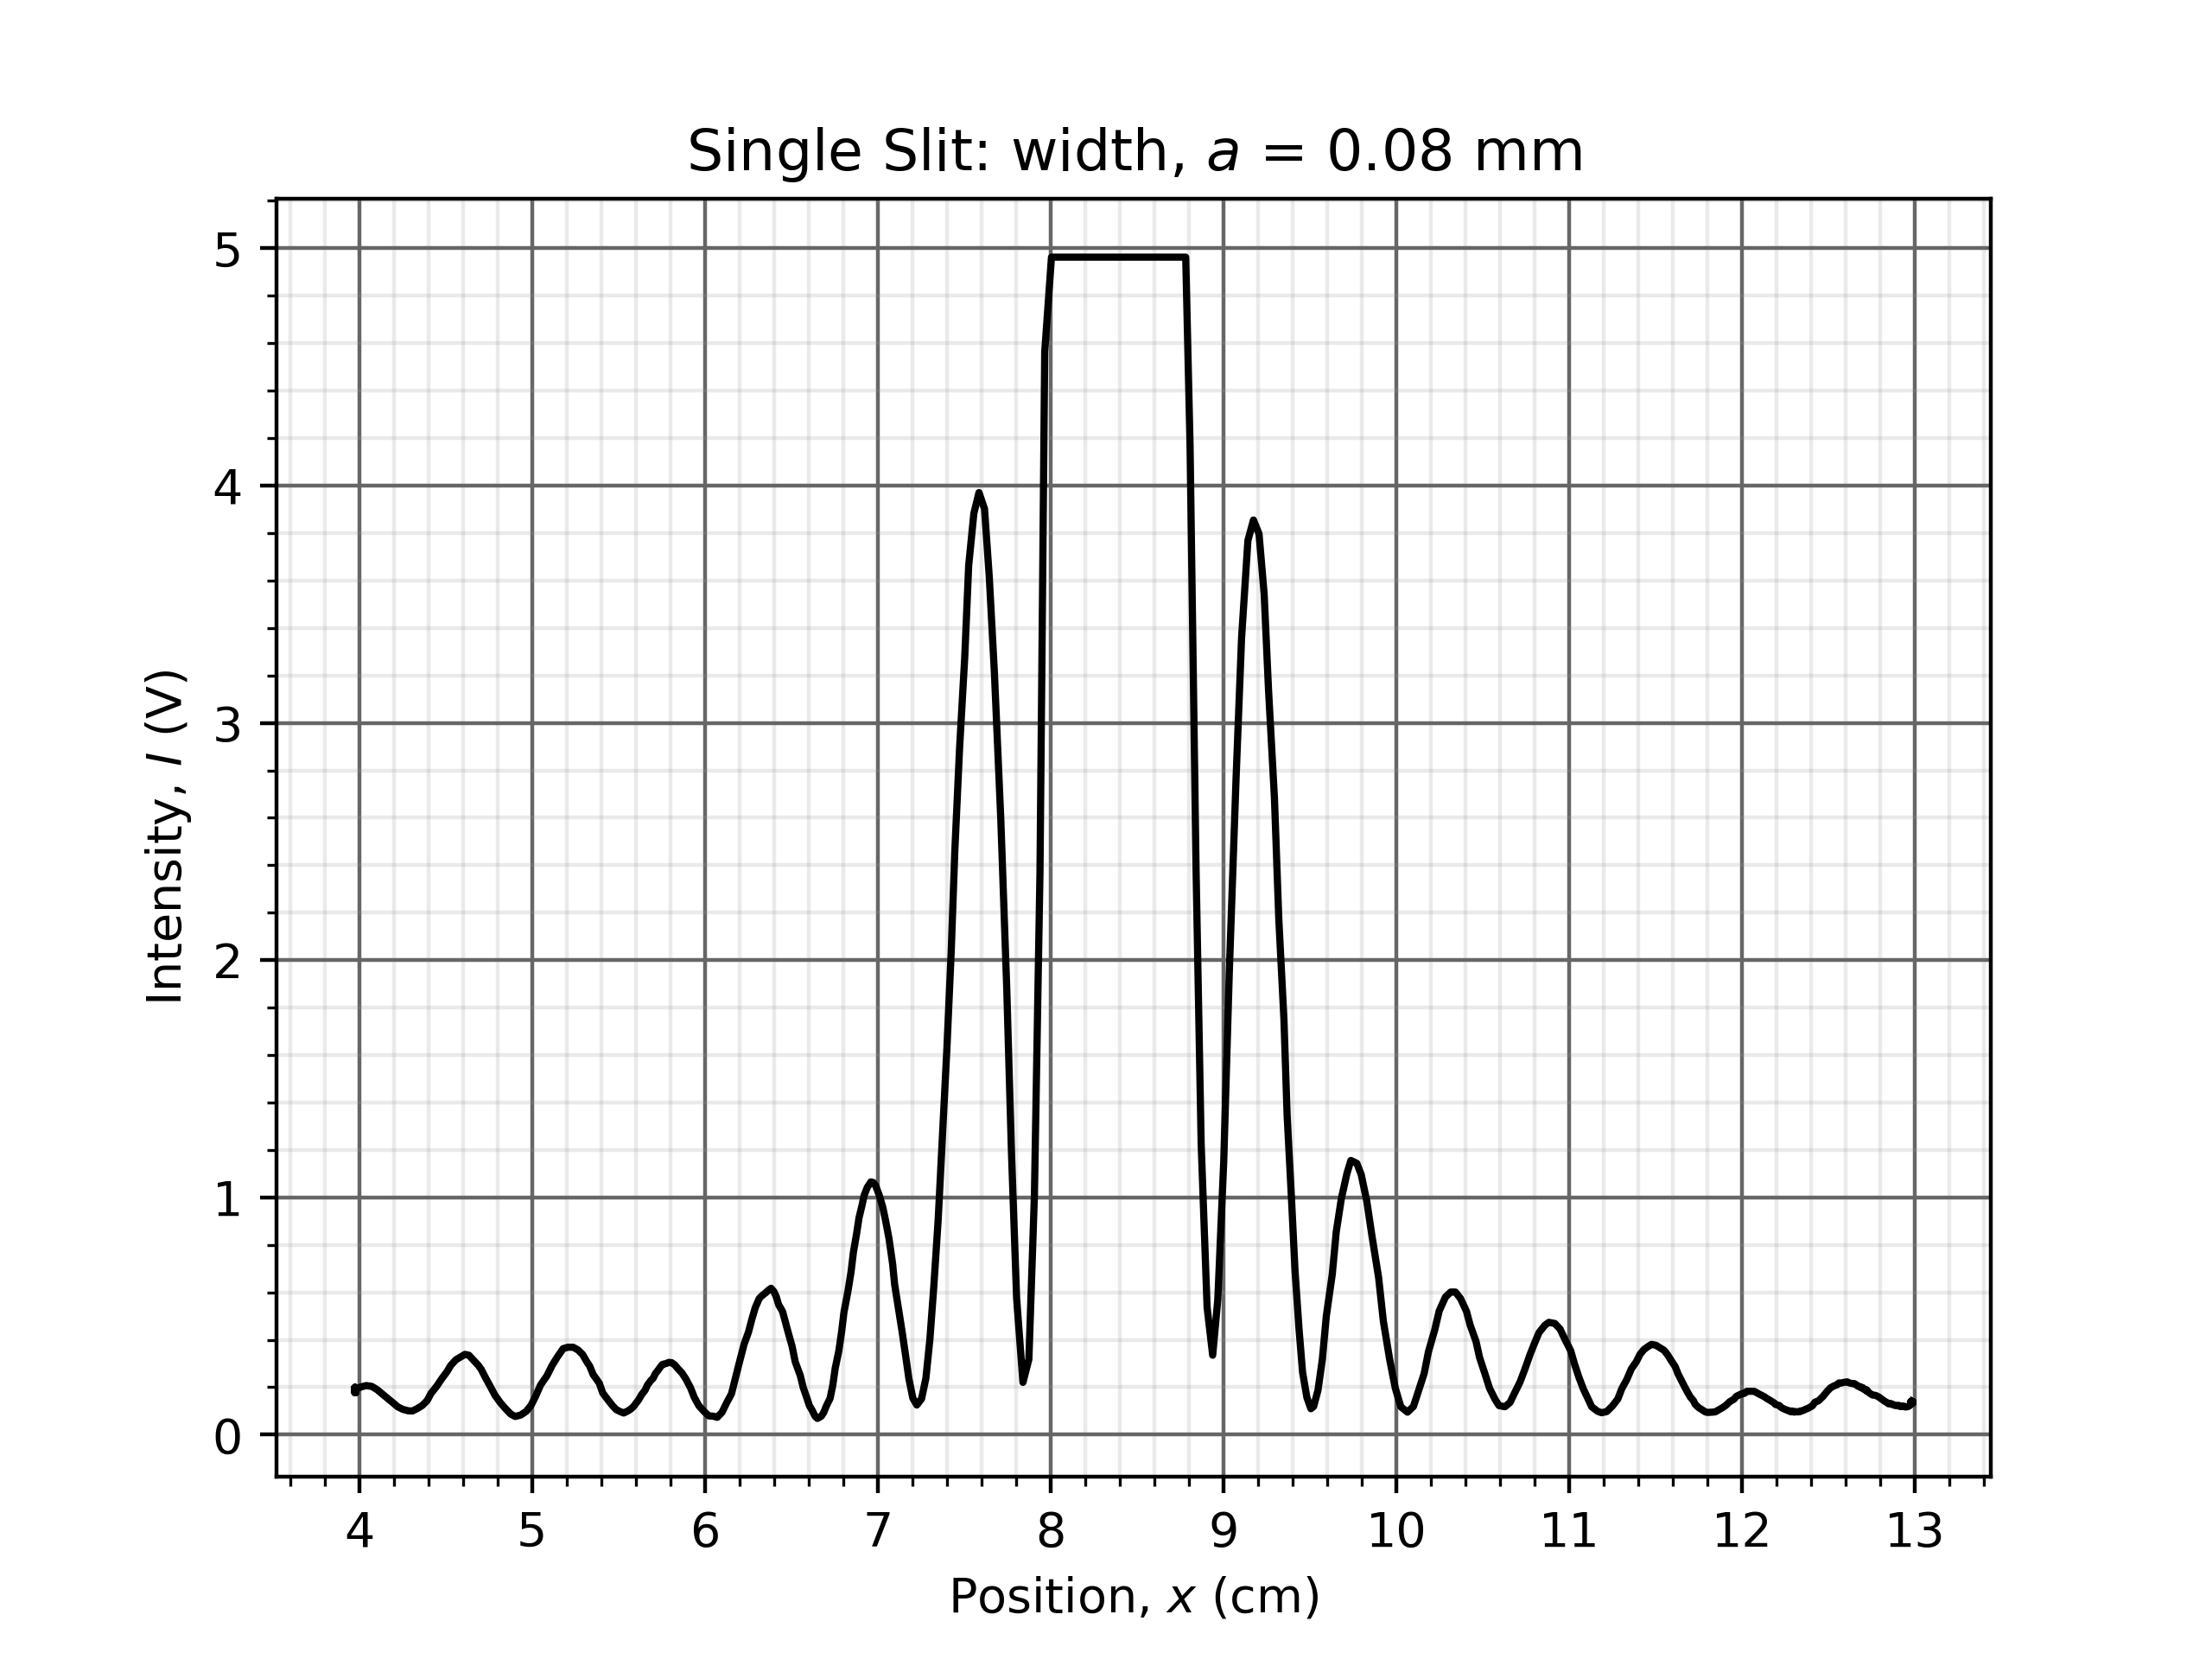
\includegraphics[width=0.4\linewidth]{../../ExtFiles/SingleSlitDiffraction.png}
    \caption{Single slit, zoomed-in.}
    \label{fig:singleSlitDiffraction}
\end{figure}\par
\textbf{Data}:
\begin{table}[h!]
    \centering
    \renewcommand{\arraystretch}{1.4}
    \begin{tabular}{|c|c|c|c|c|c|}
        \hline
        $n$ & $x_\text{min,left}$ ($\si{\centi\meter}$) & $x_\text{min,right}$ ($\si{\centi\meter}$) & $x_\text{min}=\frac{x_\text{min,right}-x_\text{min,left}}{2}$ ($\si{\centi\meter}$) & $\sin\theta_\text{min}$ & $a\sin\theta_\text{min}$ ($\si{\micro\meter}$)\\
        \hline
        1 & 7.8 & 9.0 & 0.60 & 0.0085 & 0.68\\
        \hline
        2 & 7.2 & 9.5 & 1.2 & 0.017 & 1.4\\
        \hline
        3 & 6.6 & 10.1 & 1.8 & 0.026 & 2.0\\
        \hline
        4 & 6.0 & 10.6 & 2.3 & 0.034 & 2.7\\
        \hline
    \end{tabular}
    \caption{Diffraction order vs. distance from the central diffraction maximum.}
    \label{fig:exp2data}
\end{table}\par
\textbf{Analysis}:\\
Since $a\sin\theta=n\lambda$, we have that
\begin{align*}
    \lambda &= \frac{\sum_{i=1}^4a\sin\theta_i}{\sum_{i=1}^4i}\\
    &= \SI{680}{\nano\meter}
\end{align*}
Additionally, we have from the formula that
\begin{align*}
    \delta\lambda &= \frac{2\delta x_\text{min,left}}{x_\text{min}}\cdot\lambda\\
    &= \frac{2\cdot 0.2}{0.6}\cdot 680\\
    &= \SI{453}{\nano\meter}
\end{align*}
Therefore, we can say that the wavelength of the light is
\begin{equation*}
    \lambda = 680\pm\SI{453}{\nano\meter}
\end{equation*}



\section{Diffraction Grating Analysis}
\textbf{Materials}: I analyzed the following image.
\begin{figure}[H]
    \centering
    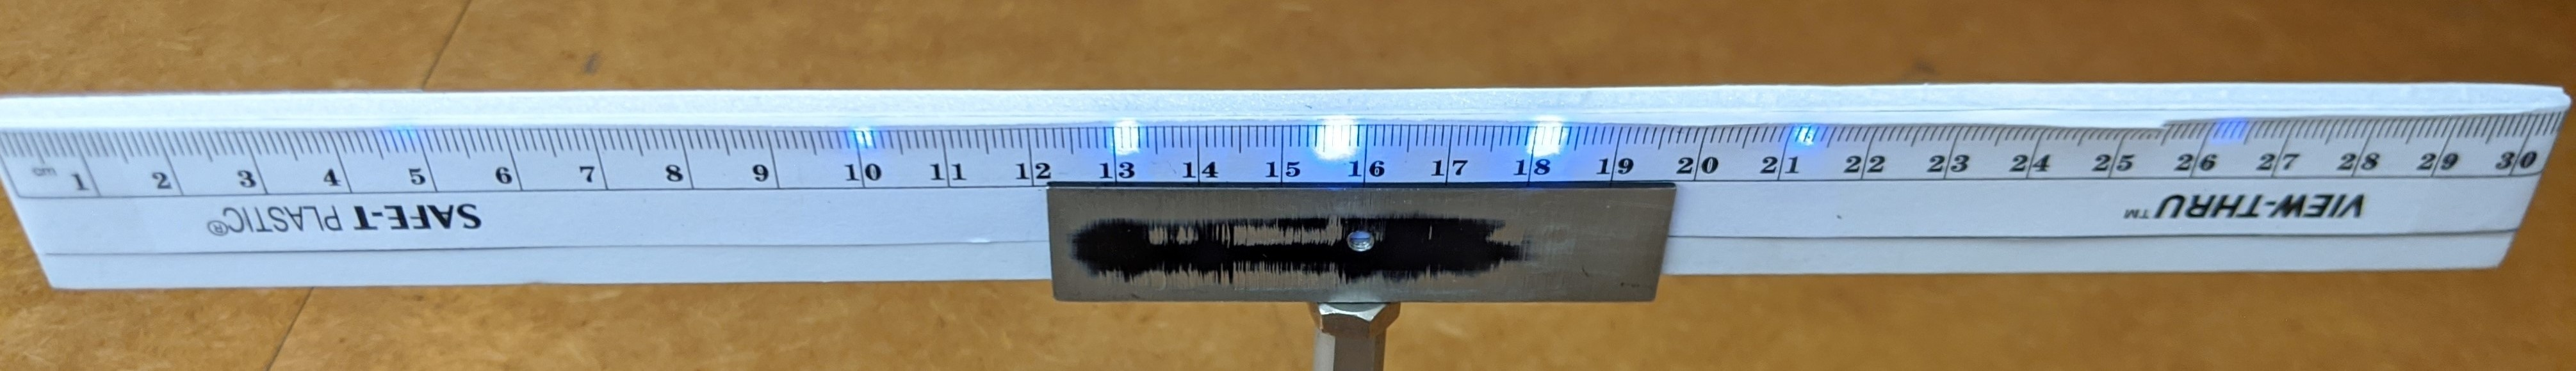
\includegraphics[width=0.9\linewidth]{../../ExtFiles/DiffractionGratingBlue.jpeg}
    \caption{Diffraction pattern for blue light.}
    \label{fig:diffractionGratingBlue}
\end{figure}\par
\textbf{Data}:
\begin{table}[h!]
    \centering
    \renewcommand{\arraystretch}{1.4}
    \begin{tabular}{|c|c|c|c|c|c|}
        \hline
        $n$ & $x_\text{min,left}$ ($\si{\centi\meter}$) & $x_\text{min,right}$ ($\si{\centi\meter}$) & $x_\text{min}=\frac{x_\text{min,right}-x_\text{min,left}}{2}$ ($\si{\centi\meter}$) & $\sin\theta_\text{min}$ & $a\sin\theta_\text{min}$ ($\si{\micro\meter}$)\\
        \hline
        1 & 13.1 & 18.1 & 2.5   & 0.247 & 0.412\\
        \hline
        2 & 10.1 & 21.2 & 5.55  & 0.493 & 0.823\\
        \hline
        3 & 4.8  & 26.3 & 10.75 & 0.739 & 1.23\\
        \hline
    \end{tabular}
    \caption{Diffraction order vs. distance from the central diffraction maximum.}
    \label{fig:exp3data}
\end{table}\par
\textbf{Analysis}:\\
Since $a\sin\theta=n\lambda$, we have that
\begin{align*}
    \lambda &= \frac{\sum_{i=1}^3a\sin\theta_i}{\sum_{i=1}^3i}\\
    &= \SI{411}{\nano\meter}
\end{align*}
Additionally, we have from the formula that
\begin{align*}
    \delta\lambda &= \frac{2\delta x_\text{min,left}}{x_\text{min}}\cdot\lambda\\
    &= \frac{2\cdot 0.1}{2.5}\cdot 411\\
    &= \SI{33}{\nano\meter}
\end{align*}
Therefore, we can say that the wavelength of the light is
\begin{equation*}
    \lambda = 411\pm\SI{33}{\nano\meter}
\end{equation*}




\end{document}